%%%%%%%%%%%%%%%%%%%%%%%%%%%%%%%%%%%%%%%%%
% Beamer Presentation
% LaTeX Template
% Version 1.0 (10/11/12)
%
% This template has been downloaded from:
% http://www.LaTeXTemplates.com
%
% License:
% CC BY-NC-SA 3.0 (http://creativecommons.org/licenses/by-nc-sa/3.0/)
%
%%%%%%%%%%%%%%%%%%%%%%%%%%%%%%%%%%%%%%%%%

%----------------------------------------------------------------------------------------
%	PACKAGES AND THEMES
%----------------------------------------------------------------------------------------

\documentclass{beamer}

\mode<presentation> {

% The Beamer class comes with a number of default slide themes
% which change the colors and layouts of slides. Below this is a list
% of all the themes, uncomment each in turn to see what they look like.

%\usetheme{default}
%\usetheme{AnnArbor}
%\usetheme{Antibes}
%\usetheme{Bergen}
%\usetheme{Berkeley}
%\usetheme{Berlin}
%\usetheme{Boadilla}
%\usetheme{CambridgeUS}
%\usetheme{Copenhagen}
%\usetheme{Darmstadt}
%\usetheme{Dresden}
%\usetheme{Frankfurt}
%\usetheme{Goettingen}
%\usetheme{Hannover}
%\usetheme{Ilmenau}
%\usetheme{JuanLesPins}
%\usetheme{Luebeck}
%\usetheme{Madrid}
%\usetheme{Malmoe}
%\usetheme{Marburg}
%\usetheme{Montpellier}
%\usetheme{PaloAlto}
\usetheme{Pittsburgh}
%\usetheme{Rochester}
%\usetheme{Singapore}
%\usetheme{Szeged}
%\usetheme{Warsaw}

% As well as themes, the Beamer class has a number of color themes
% for any slide theme. Uncomment each of these in turn to see how it
% changes the colors of your current slide theme.

%\usecolortheme{albatross}
%\usecolortheme{beaver}
%\usecolortheme{beetle}
%\usecolortheme{crane}
%\usecolortheme{dolphin}
%\usecolortheme{dove}
%\usecolortheme{fly}
%\usecolortheme{lily}
%\usecolortheme{orchid}
%\usecolortheme{rose}
%\usecolortheme{seagull}
%\usecolortheme{seahorse}
%\usecolortheme{whale}
%\usecolortheme{wolverine}

%\setbeamertemplate{footline} % To remove the footer line in all slides uncomment this line
\setbeamertemplate{footline}[page number] % To replace the footer line in all slides with a simple slide count uncomment this line

\setbeamertemplate{navigation symbols}{} % To remove the navigation symbols from the bottom of all slides uncomment this line
}

\AtBeginSection{\frame{\sectionpage}}

\usepackage{graphicx} % Allows including images
\graphicspath{ {../img/} }
\usepackage{booktabs} % Allows the use of \toprule, \midrule and \bottomrule in tables
\usepackage{csquotes}

%----------------------------------------------------------------------------------------
%	TITLE PAGE
%----------------------------------------------------------------------------------------

\title[]{Applied Econometrics for Fun and Profit} % The short title appears at the bottom of every slide, the full title is only on the title page

\author{Sahil Chinoy} % Your name
\institute % Your institution as it will appear on the bottom of every slide, may be shorthand to save space
{
 \\ % Your institution for the title page
}
\date{July 26, 2017} % Date, can be changed to a custom date

\begin{document}

\begin{frame}
\titlepage % Print the title page as the first slide
\end{frame}

\begin{frame}
% Table of contents slide, comment this block out to remove it
\tableofcontents % Throughout your presentation, if you choose to use \section{} and \subsection{} commands, these will automatically be printed on this slide as an overview of your presentation
\end{frame}

%----------------------------------------------------------------------------------------
%	PRESENTATION SLIDES
%----------------------------------------------------------------------------------------

%------------------------------------------------
\section{Why bother?}

\begin{frame}
	\begin{itemize}
		\item Economists and academics are bad at many things. One of them is graphics.
	\end{itemize}
	\begin{figure}
		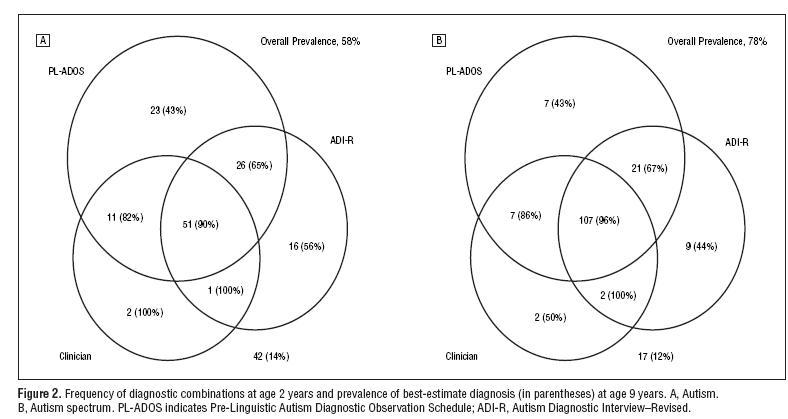
\includegraphics[width=8cm]{autism-test-figure-21.jpg}
		\centering
	\end{figure}
\end{frame}

\begin{frame}
	\begin{itemize}
		\item But they are good at two things that journalists can learn.
		\begin{itemize}
			\item Causal inference.
			\item Quantifying uncertainty.
		\end{itemize}
		\item Why should you care?
		\begin{itemize}
			\item Dissect studies.
			\item Talk to academics in their language.
			\item Use econometric tools in your own reporting.
		\end{itemize}
	\end{itemize}
\end{frame}

\begin{frame}
	\begin{itemize}
		\item The standard tool of econometrics is the ordinary least-squares (linear) regression. It's useful and well-understood.
		\begin{itemize}
			\item But it's easy to abuse to find spurious correlations.\footnote{\url{http://www.tylervigen.com/spurious-correlations}}
			\item Also, it's a little boring. 
		\end{itemize}
	\end{itemize}
	\begin{figure}
		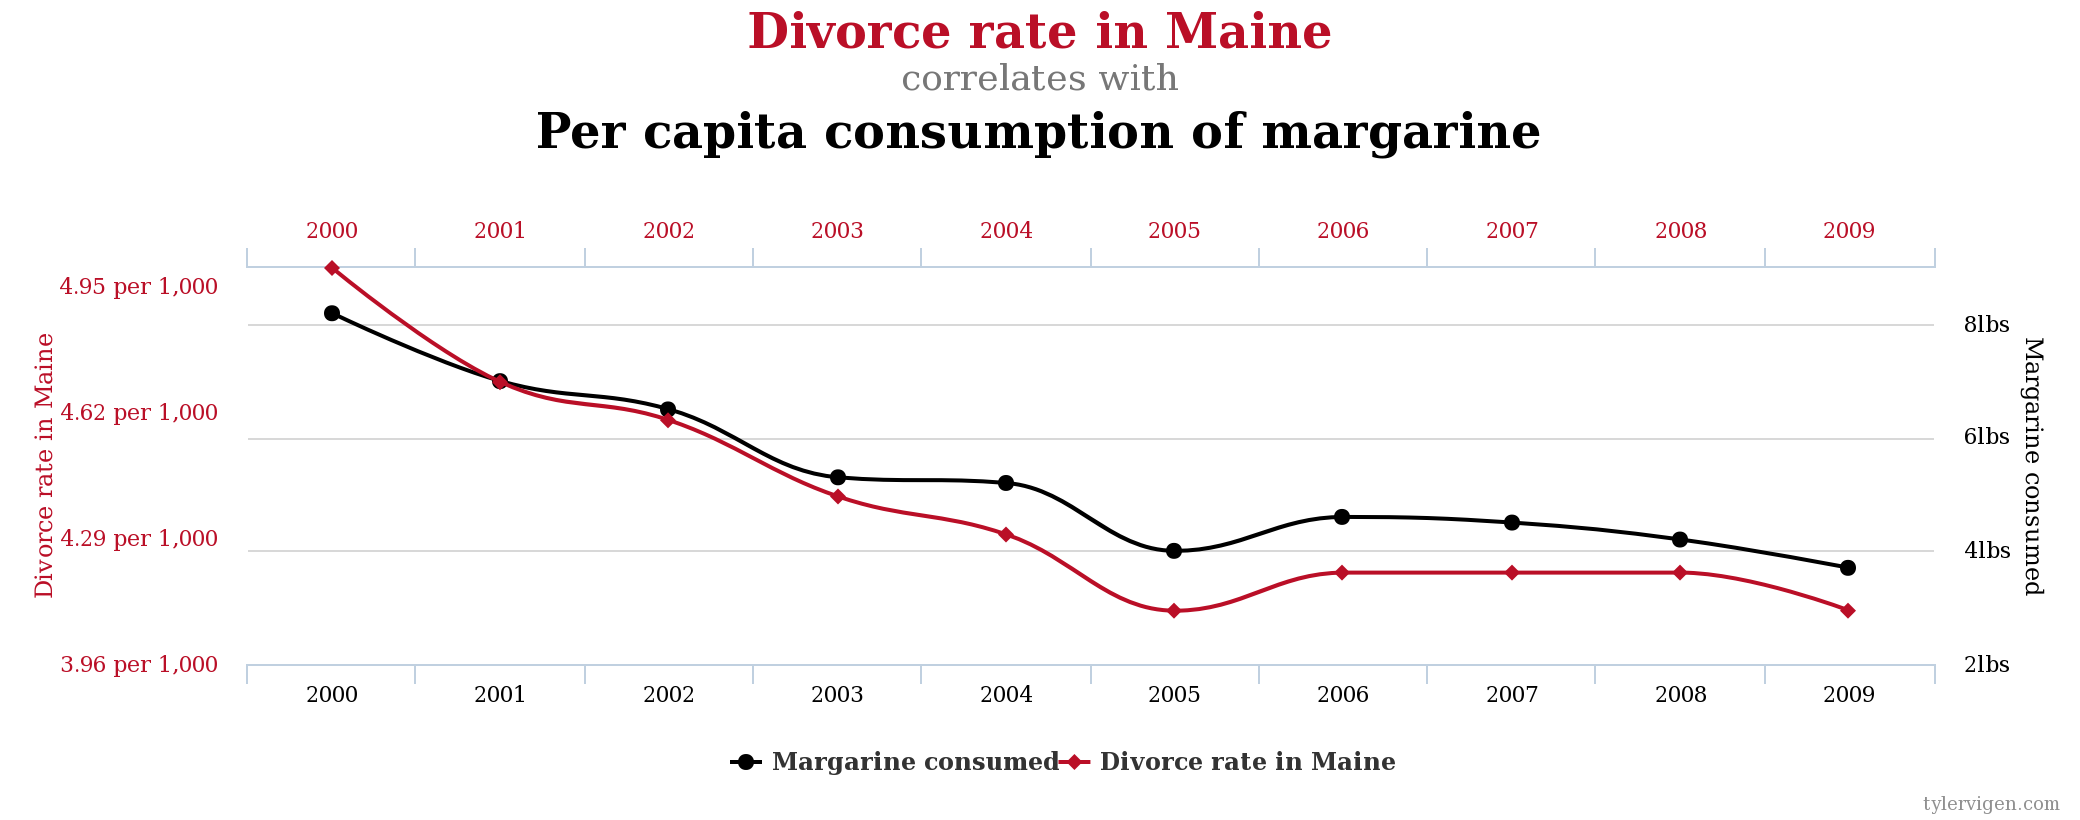
\includegraphics[width=10cm]{spurious-correlations.png}
		\centering
	\end{figure}
\end{frame}

\begin{frame}
	\begin{itemize}
	\item Today, we'll run through three other techniques in applied econometrics.
		\begin{itemize}
			\item This will be focused on examples, not theory or coding.
			\item It's intended to help you get familiar with the terminology, understand what's possible and know how to get started.
		\end{itemize}
	\end{itemize}
\end{frame}

\section{Regression discontinuity}

\begin{frame}
	\begin{itemize}
	\item Like researchers, we're often after causality. It's a better story to say that X causes Y, not just that X and Y are related.
	\item The gold standard: randomized trials. 
		\begin{itemize}
			\item Think military drafts. Because whether you're drafted is essentially random, we can use the difference in outcomes between the two groups to analyze the causal effect of joining the military.
		\end{itemize}
	\item Often in real life, we don't have that kind of randomness.\footnote{For example, we can't randomly give aid to some poor nations but not others.}
	\item So, we take some sort of cutoff, and assume that if you're close to the cutoff, which side you're on is \textit{basically} random.
	\end{itemize}
\end{frame}

\begin{frame}
	\begin{itemize}
		\item Here's the classic example.\footnote{More examples in \cite{lee2010regression}, pp. 339-42.}
		\begin{itemize}
			\item Say that if you get a 2000 or above on your SAT, you're guaranteed to get into college, but if you get below 2000, you don't.
			\item The difference in ability between someone who scores 1980 and 2020 is basically nothing.
			\item So we can use the difference in the earnings of people who scored below 2000 and above 2000 to get the causal effect of college admission on earnings.
		\end{itemize}
	\end{itemize}
	\begin{figure}
		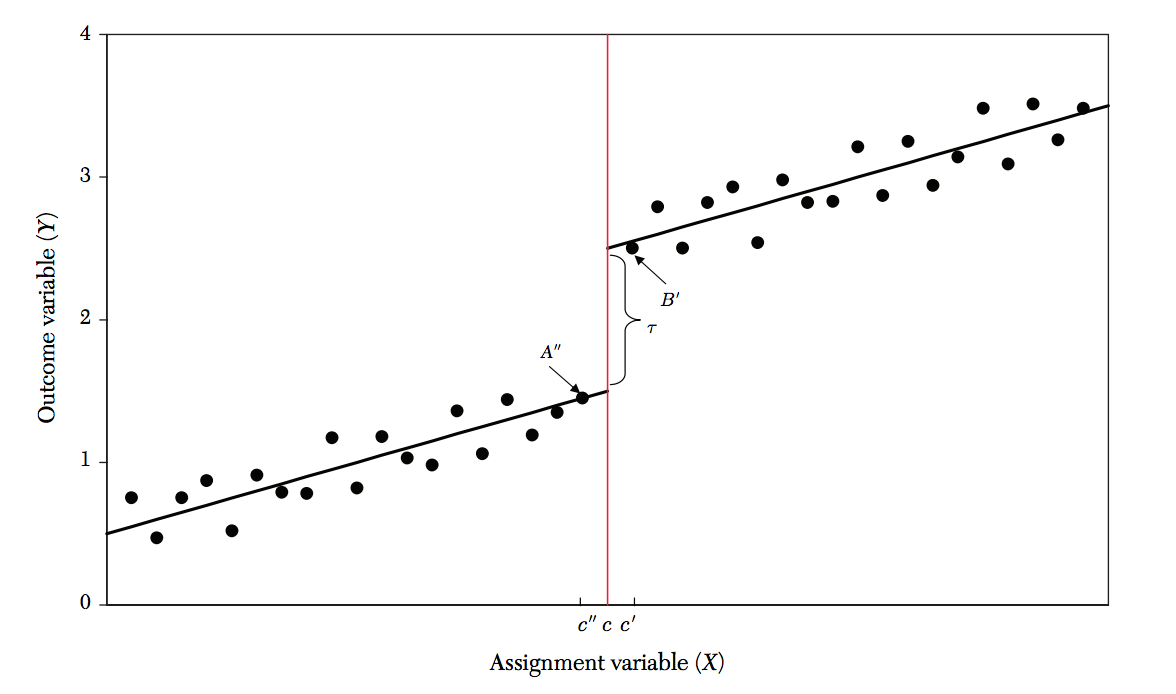
\includegraphics[width=6cm]{lee-rd.png}
		\centering
	\end{figure}
\end{frame}

\begin{frame}
	\begin{itemize}
		\item Discontinuities due to policy or custom.\footnote{See \cite{angrist1999using}.}
		\begin{itemize}
			\item The maximum number of students per teacher in Israel is 40.
			\item But a cohort with 40 students is basically the same as a cohort of 41 students except for how many teachers they have.
			\item This can be used to get the causal effect of classroom size on test scores.
		\end{itemize}
	\end{itemize}
	\begin{figure}
		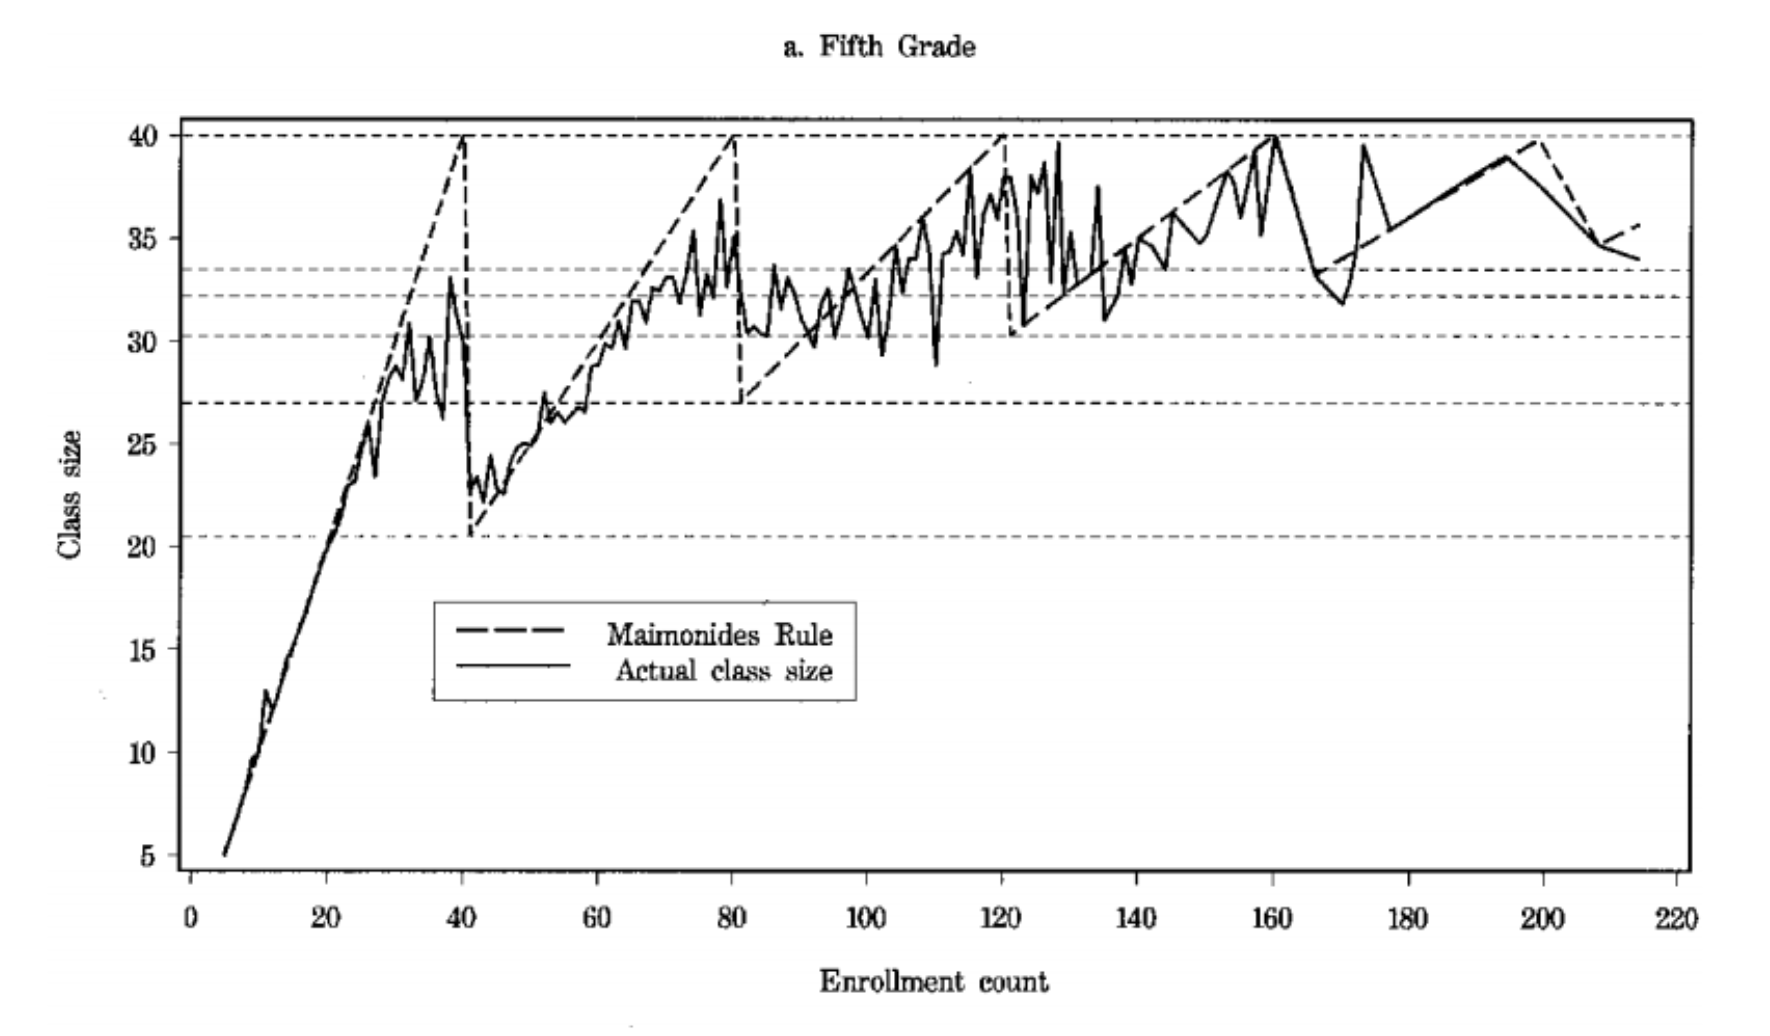
\includegraphics[width=8cm]{angrist-maimonedes.png}
		\centering
	\end{figure}
\end{frame}

\begin{frame}
	\begin{itemize}
		\item Geographic distance from a border where some meaningful policy change happens.\footnote{See \cite{black1999better}.}
		\begin{itemize}
			\item Consider houses on two sides of a school district border. They are basically the same except for the school they're assigned to.
			\item This can be used to figure out how much parents are willing to pay to send their children to better schools.
		\end{itemize}
	\end{itemize}
	\begin{figure}
		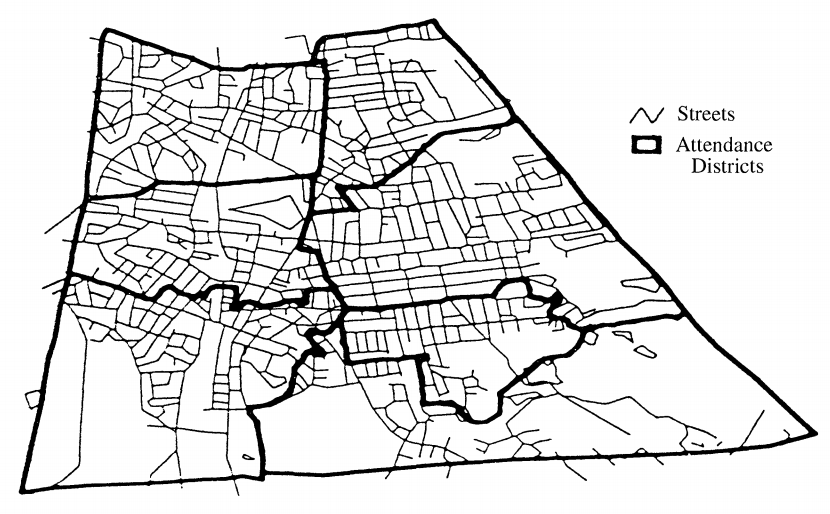
\includegraphics[width=7cm]{black-schools.png}
		\centering
	\end{figure}
\end{frame}

\begin{frame}
	\begin{itemize}
		\item How to do it
		\begin{itemize}
			\item Make a scatterplot, then draw two trend lines on either side of the cutoff.
			\item The visual discontinuity can be powerful even without the underlying statistics, but make sure the effect you observe is significant.
		\end{itemize}
	\end{itemize}
	\begin{figure}
		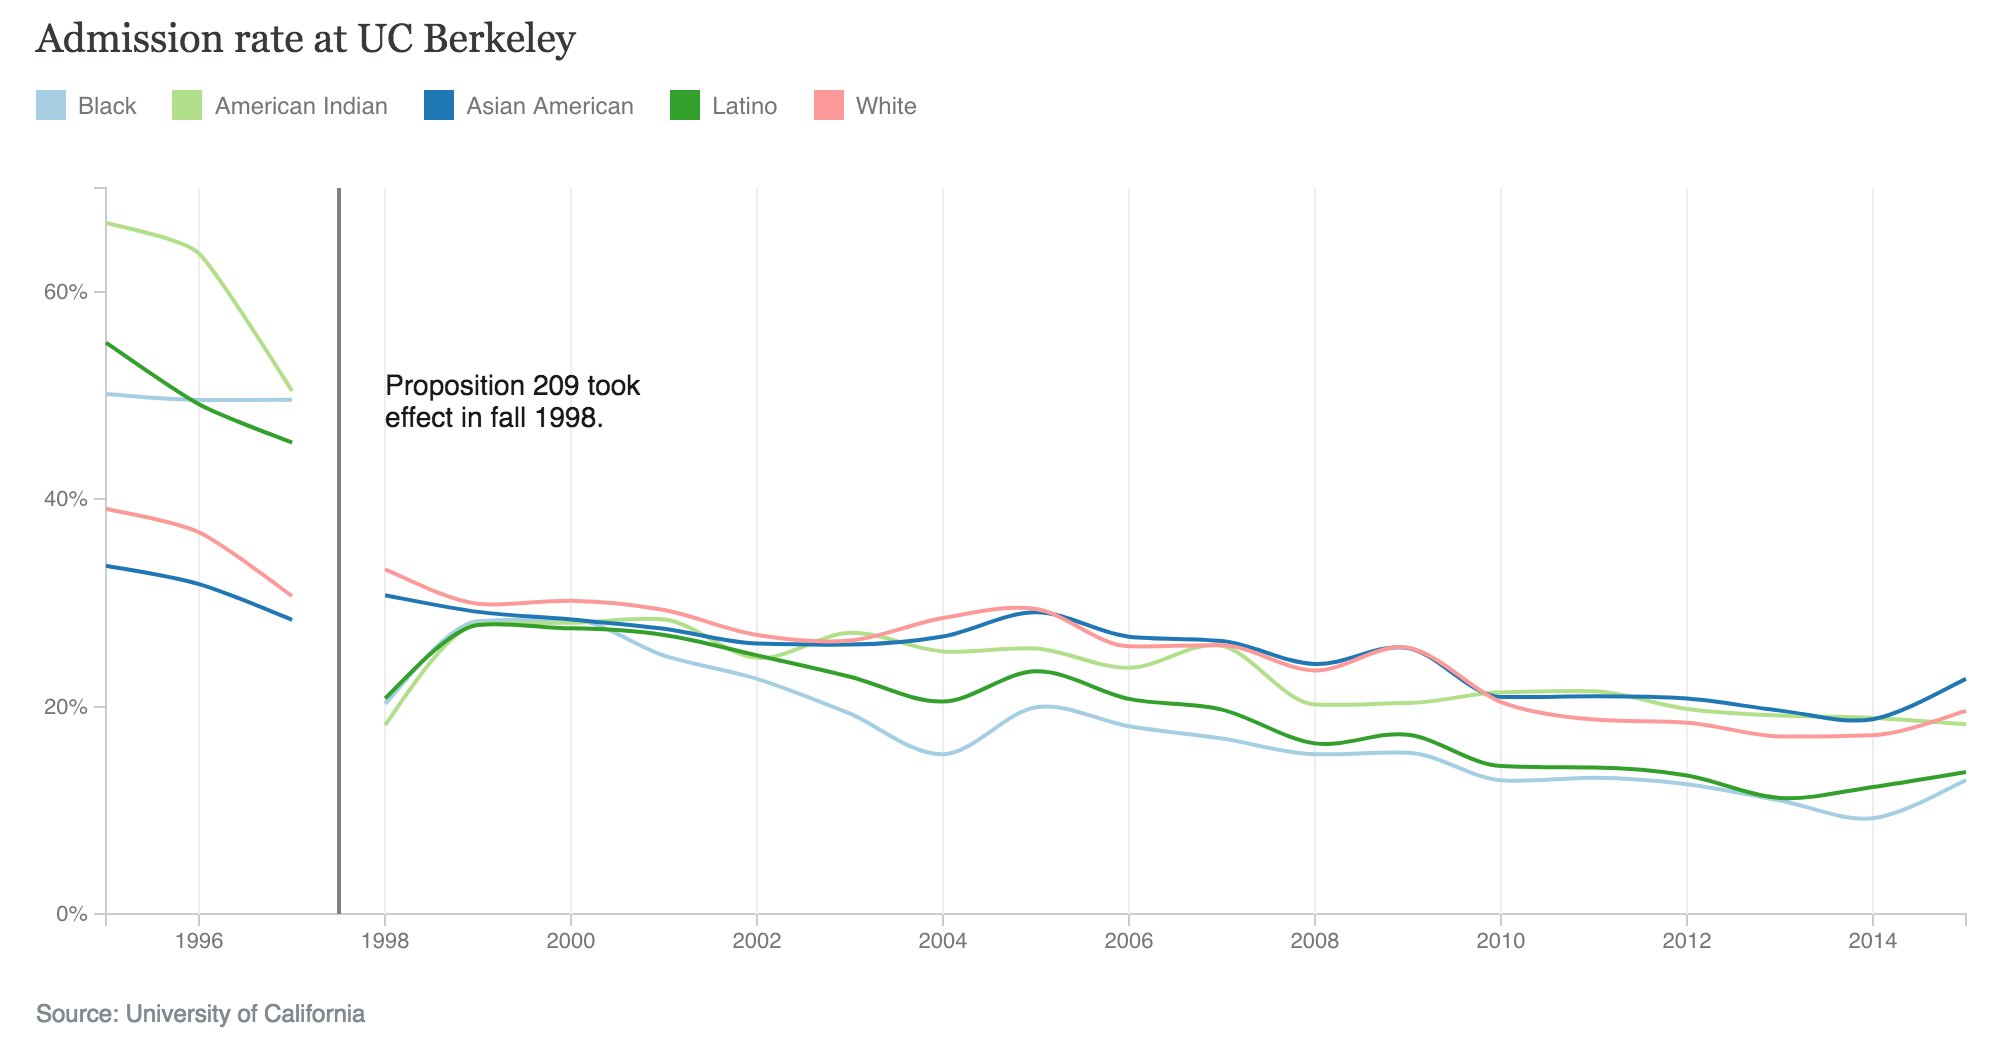
\includegraphics[width=10cm]{affirmative-action.png}
		\centering
	\end{figure}
\end{frame}

\begin{frame}
	\begin{itemize}
		\item Run a linear regression with a binary variable to indicate the side of the cutoff you're on. Then check the magnitude and significance of the coefficient.
			\begin{itemize}
				\item Python: \texttt{statsmodels.OLS}.
				\item See \url{github.com/natematias/research_in_python} for an example in a Jupyter notebook.
			\end{itemize}
	\end{itemize}
	\begin{figure}
		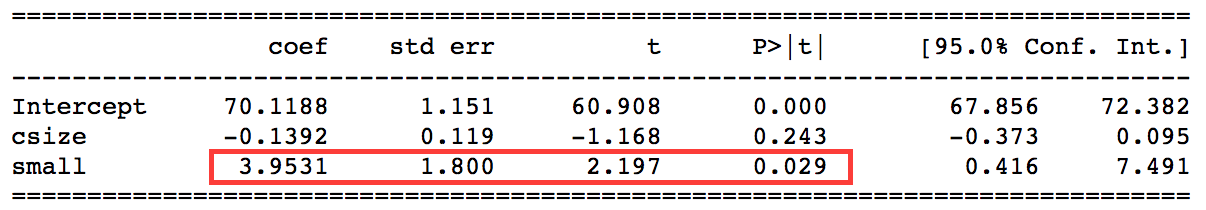
\includegraphics[width=10cm]{matias-coeff.png}
		\centering
	\end{figure}
\end{frame}

\section{Quantile regression}

\begin{frame}
	\begin{itemize}
		\item Ordinary least-squares estimates the conditional mean of a dependent variable given particular values of the independent variables.
		\item But for skewed distributions, the mean can be misleading. Sometimes the median is more informative.
		\item What if we could estimate the conditional median? Or the 25th percentile, or the 99th percentile...
		\begin{figure}
			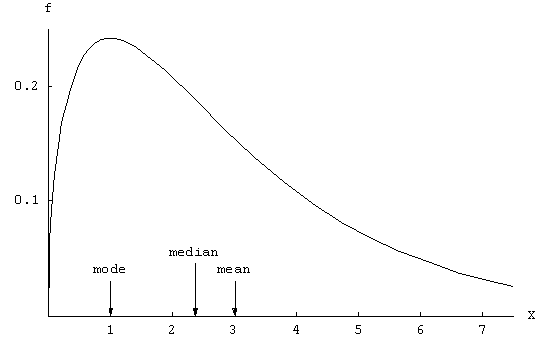
\includegraphics[width=7cm]{skewed-distribution.png}
			\centering
		\end{figure}
	\end{itemize}
\end{frame}

\begin{frame}
	\begin{itemize}
		\item Example: I want to know what to major in to boost my future earnings.
		\item First attempt: Average earnings by major.
			\begin{itemize}
				\item But men earn more on average, and engineering majors are more likely to be male.
			\end{itemize}
	\end{itemize}
	\begin{figure}
		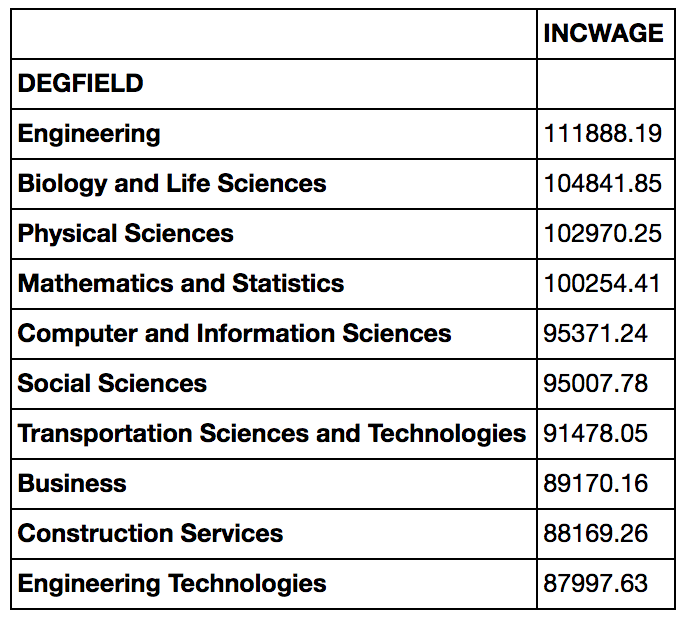
\includegraphics[width=6cm]{chinoy-majors-1.png}
		\centering
	\end{figure}
\end{frame}

\begin{frame}
	\begin{itemize}
		\item Second attempt: Linear regression to account for gender, race and age.
			\begin{itemize}
				\item “Engineering Technologies” drops out of the list because it is skewed male.
				\item Biology still appears second on the list.
				\item Doctors make a lot of money, but many biology majors end up as medical technicians.
				\item Maybe we want to look at the median earnings. Or better yet, maybe we want a fuller picture of the distribution of earnings.
			\end{itemize}
	\end{itemize}
\end{frame}

\begin{frame}
	\begin{itemize}
		\item Third attempt: Quantile regression. What is the effect on earnings \textit{at some quantile} of majoring in X (relative to some reference major), controlling for race, gender and age? 
		\begin{itemize}
			\item Earnings at the 95th percentile for biology majors look very different than the median.
		\end{itemize}
	\end{itemize}
	\begin{figure}
		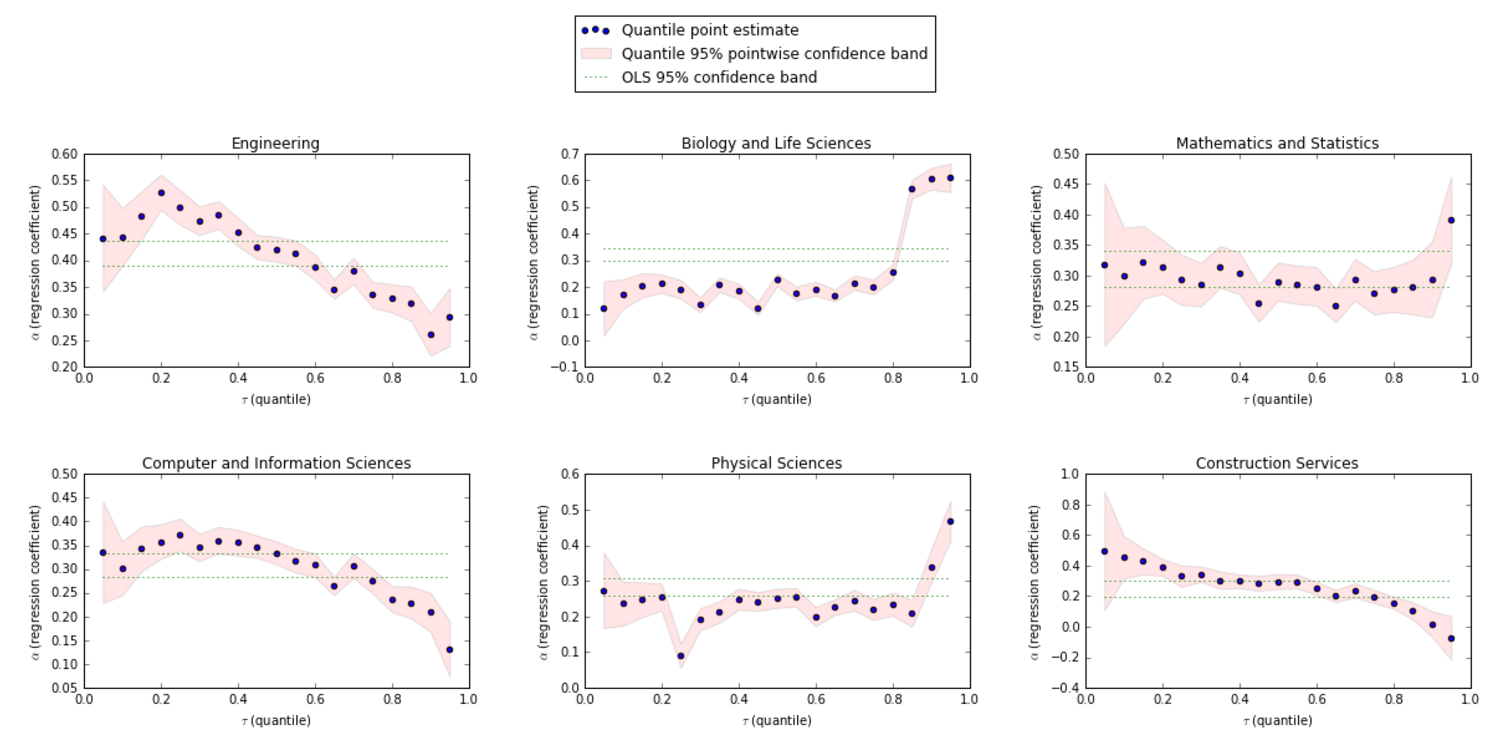
\includegraphics[width=10cm]{chinoy-majors-2.png}
		\centering
	\end{figure}
\end{frame}

\begin{frame}
	\begin{itemize}
		\item Effect of mother's race on birthweight.\footnote{See \cite{koenker2001quantile}.}
		\begin{itemize}
			\item At the lowest quantiles, babies born to black mothers weigh 300 g less than those born to white mothers. At the top quantiles, the difference is more like 150 g. 
		\end{itemize}
	\end{itemize}
	\begin{figure}
		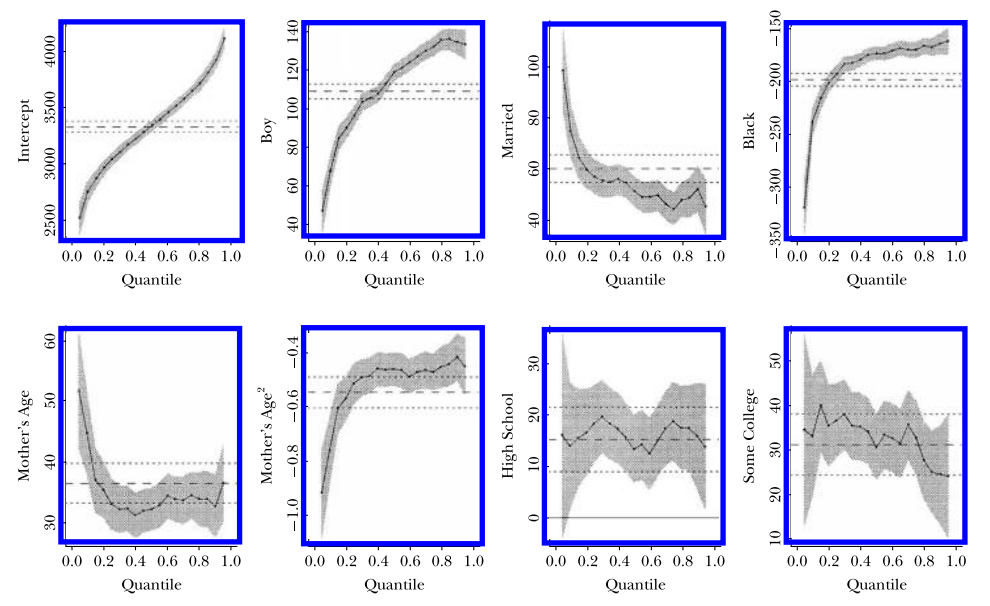
\includegraphics[width=8cm]{koenker-birthweight.png}
		\centering
	\end{figure}
\end{frame}

\begin{frame}
	\begin{itemize}
		\item Ethnicity and wealth across 19th-century American cities.\footnote{See \cite{conley1998nativity}.}
		\begin{itemize}
			\item At the lowest quantiles, German workers in Indianapolis are far wealthier than others. At the top quantiles, this effect disappears. 
		\end{itemize}
	\end{itemize}
	\begin{figure}
		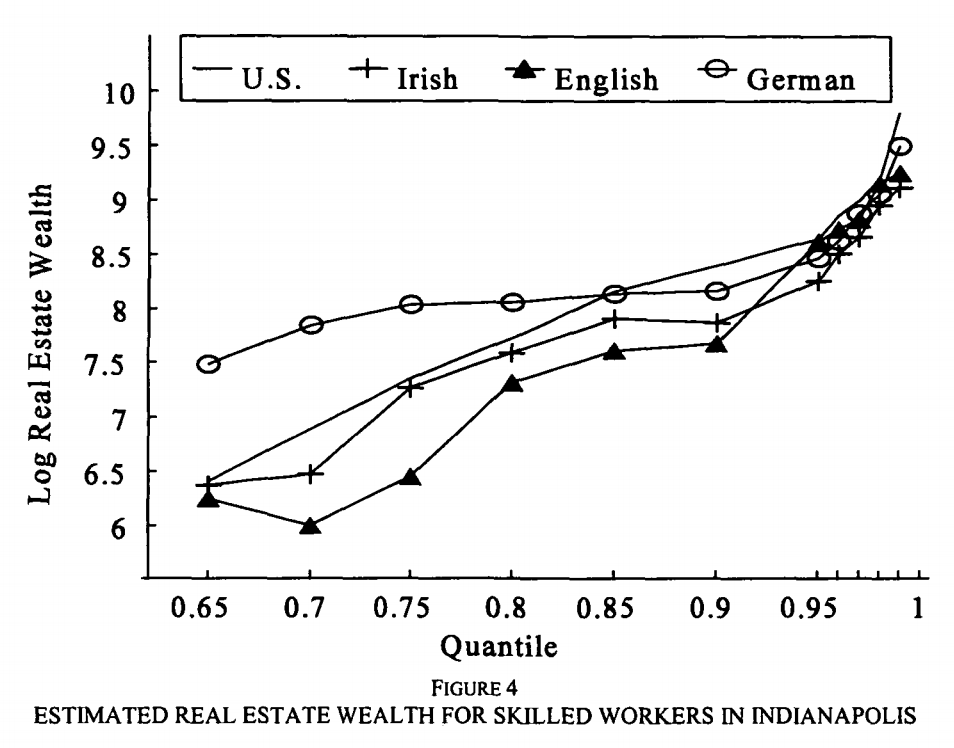
\includegraphics[width=6cm]{conley-realestate.png}
		\centering
	\end{figure}
\end{frame} 

\begin{frame}
	\begin{itemize}
		\item Effect of unions on wages.\footnote{See \cite{chamberlain1994quantile}.}
		\begin{itemize}
			\item At the lowest quantiles, unions make a big difference in wages. At the top of the wage distribution, unions hardly matter. 
		\end{itemize}
	\end{itemize}
	\begin{figure}
		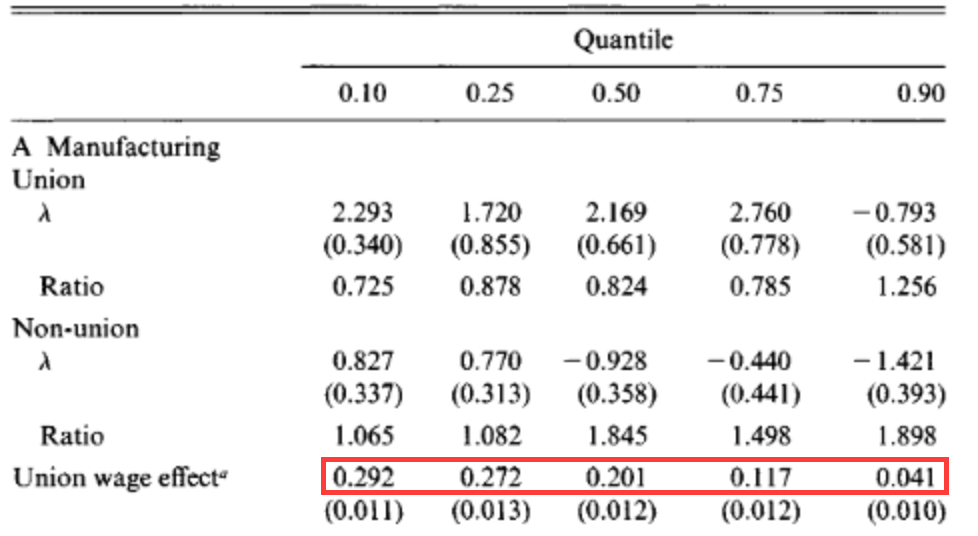
\includegraphics[width=8cm]{chamberlain-unions.png}
		\centering
	\end{figure}
\end{frame} 

\begin{frame}
	\begin{itemize}
		\item How to do it
		\begin{itemize}
			\item Pretty much like an OLS regression computed for a given quantile.
			\item Works by dividing your sample into ``cells" for each combination of the explanatory variables, so it requires a large sample size.\footnote{Sort of.}
			\item Python: \texttt{statsmodels.quantReg}.
			\item See me for the college majors example in a Jupyter notebook.
		\end{itemize}
	\end{itemize}
\end{frame}

\section{Survival analysis}

\begin{frame}
	\begin{itemize}
		\item We're interested in durations and how they differ across groups.
			\begin{itemize}
				\item Length of a politician's time in office for different parties.
				\item Patient lifetime after heart surgery for different doctors.
			\end{itemize}
		\item The problem: We don't observe the ``death'' event for every individual.
			\begin{itemize}
				\item This is known as censorship, and will lead us to underestimate the true lifetime.
			\end{itemize}
	\end{itemize}
	\begin{figure}
		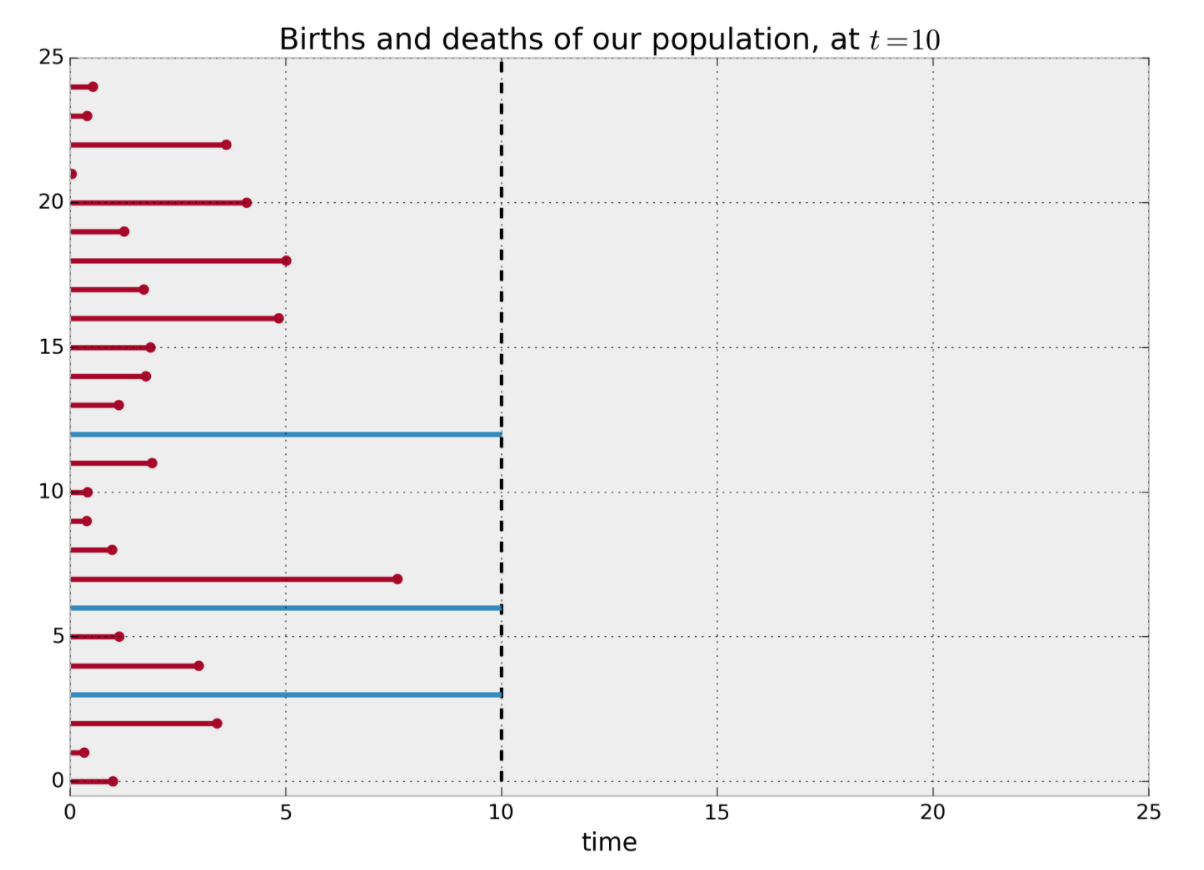
\includegraphics[width=6cm]{lifelines-censorship.png}
		\centering
	\end{figure}
\end{frame}

\begin{frame}
	\begin{itemize}
		\item Survival analysis is essentially a bag of tools to get around the censorship problem.
		\item It lets us estimate the \textit{survival function}\footnote{Known as the Kaplan-Meier estimator.} -- the fraction of the population that survives past a given time -- and the \textit{hazard rate} -- the probability of ``dying'' at a given time.
	\end{itemize}
	\begin{figure}
		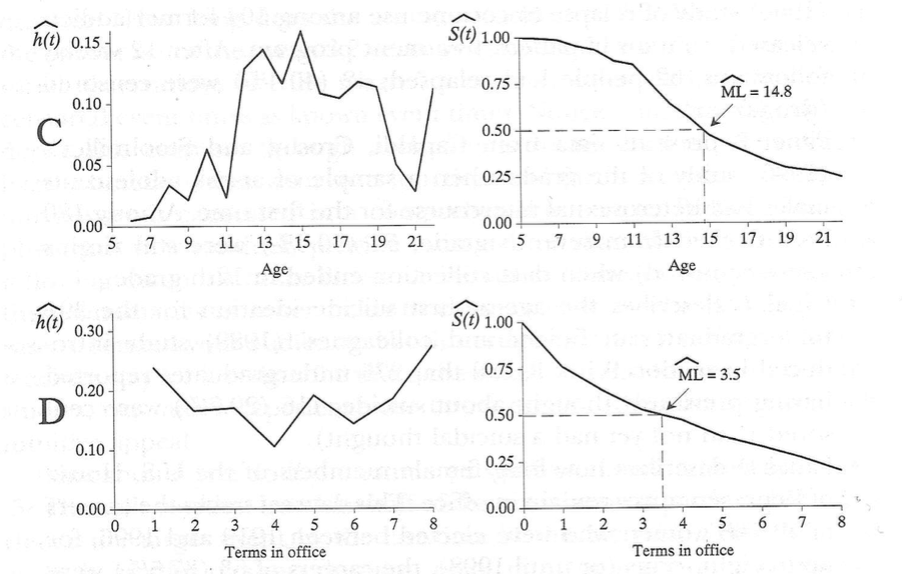
\includegraphics[width=8cm]{singer-survivalhazard.png}
		\centering
	\end{figure}
\end{frame}

\begin{frame}
	\begin{itemize}
		\item We can run a survival regression to analyze how the baseline hazard rate changes with some explanatory variable.
		\item But it's sometimes enough just to look at the survival functions for subgroups.
		\begin{itemize}
			\item Consider the lifetime for democratic and nondemocratic regimes.\footnote{\url{lifelines.readthedocs.io}}
		\end{itemize}
	\end{itemize}
	\begin{figure}
		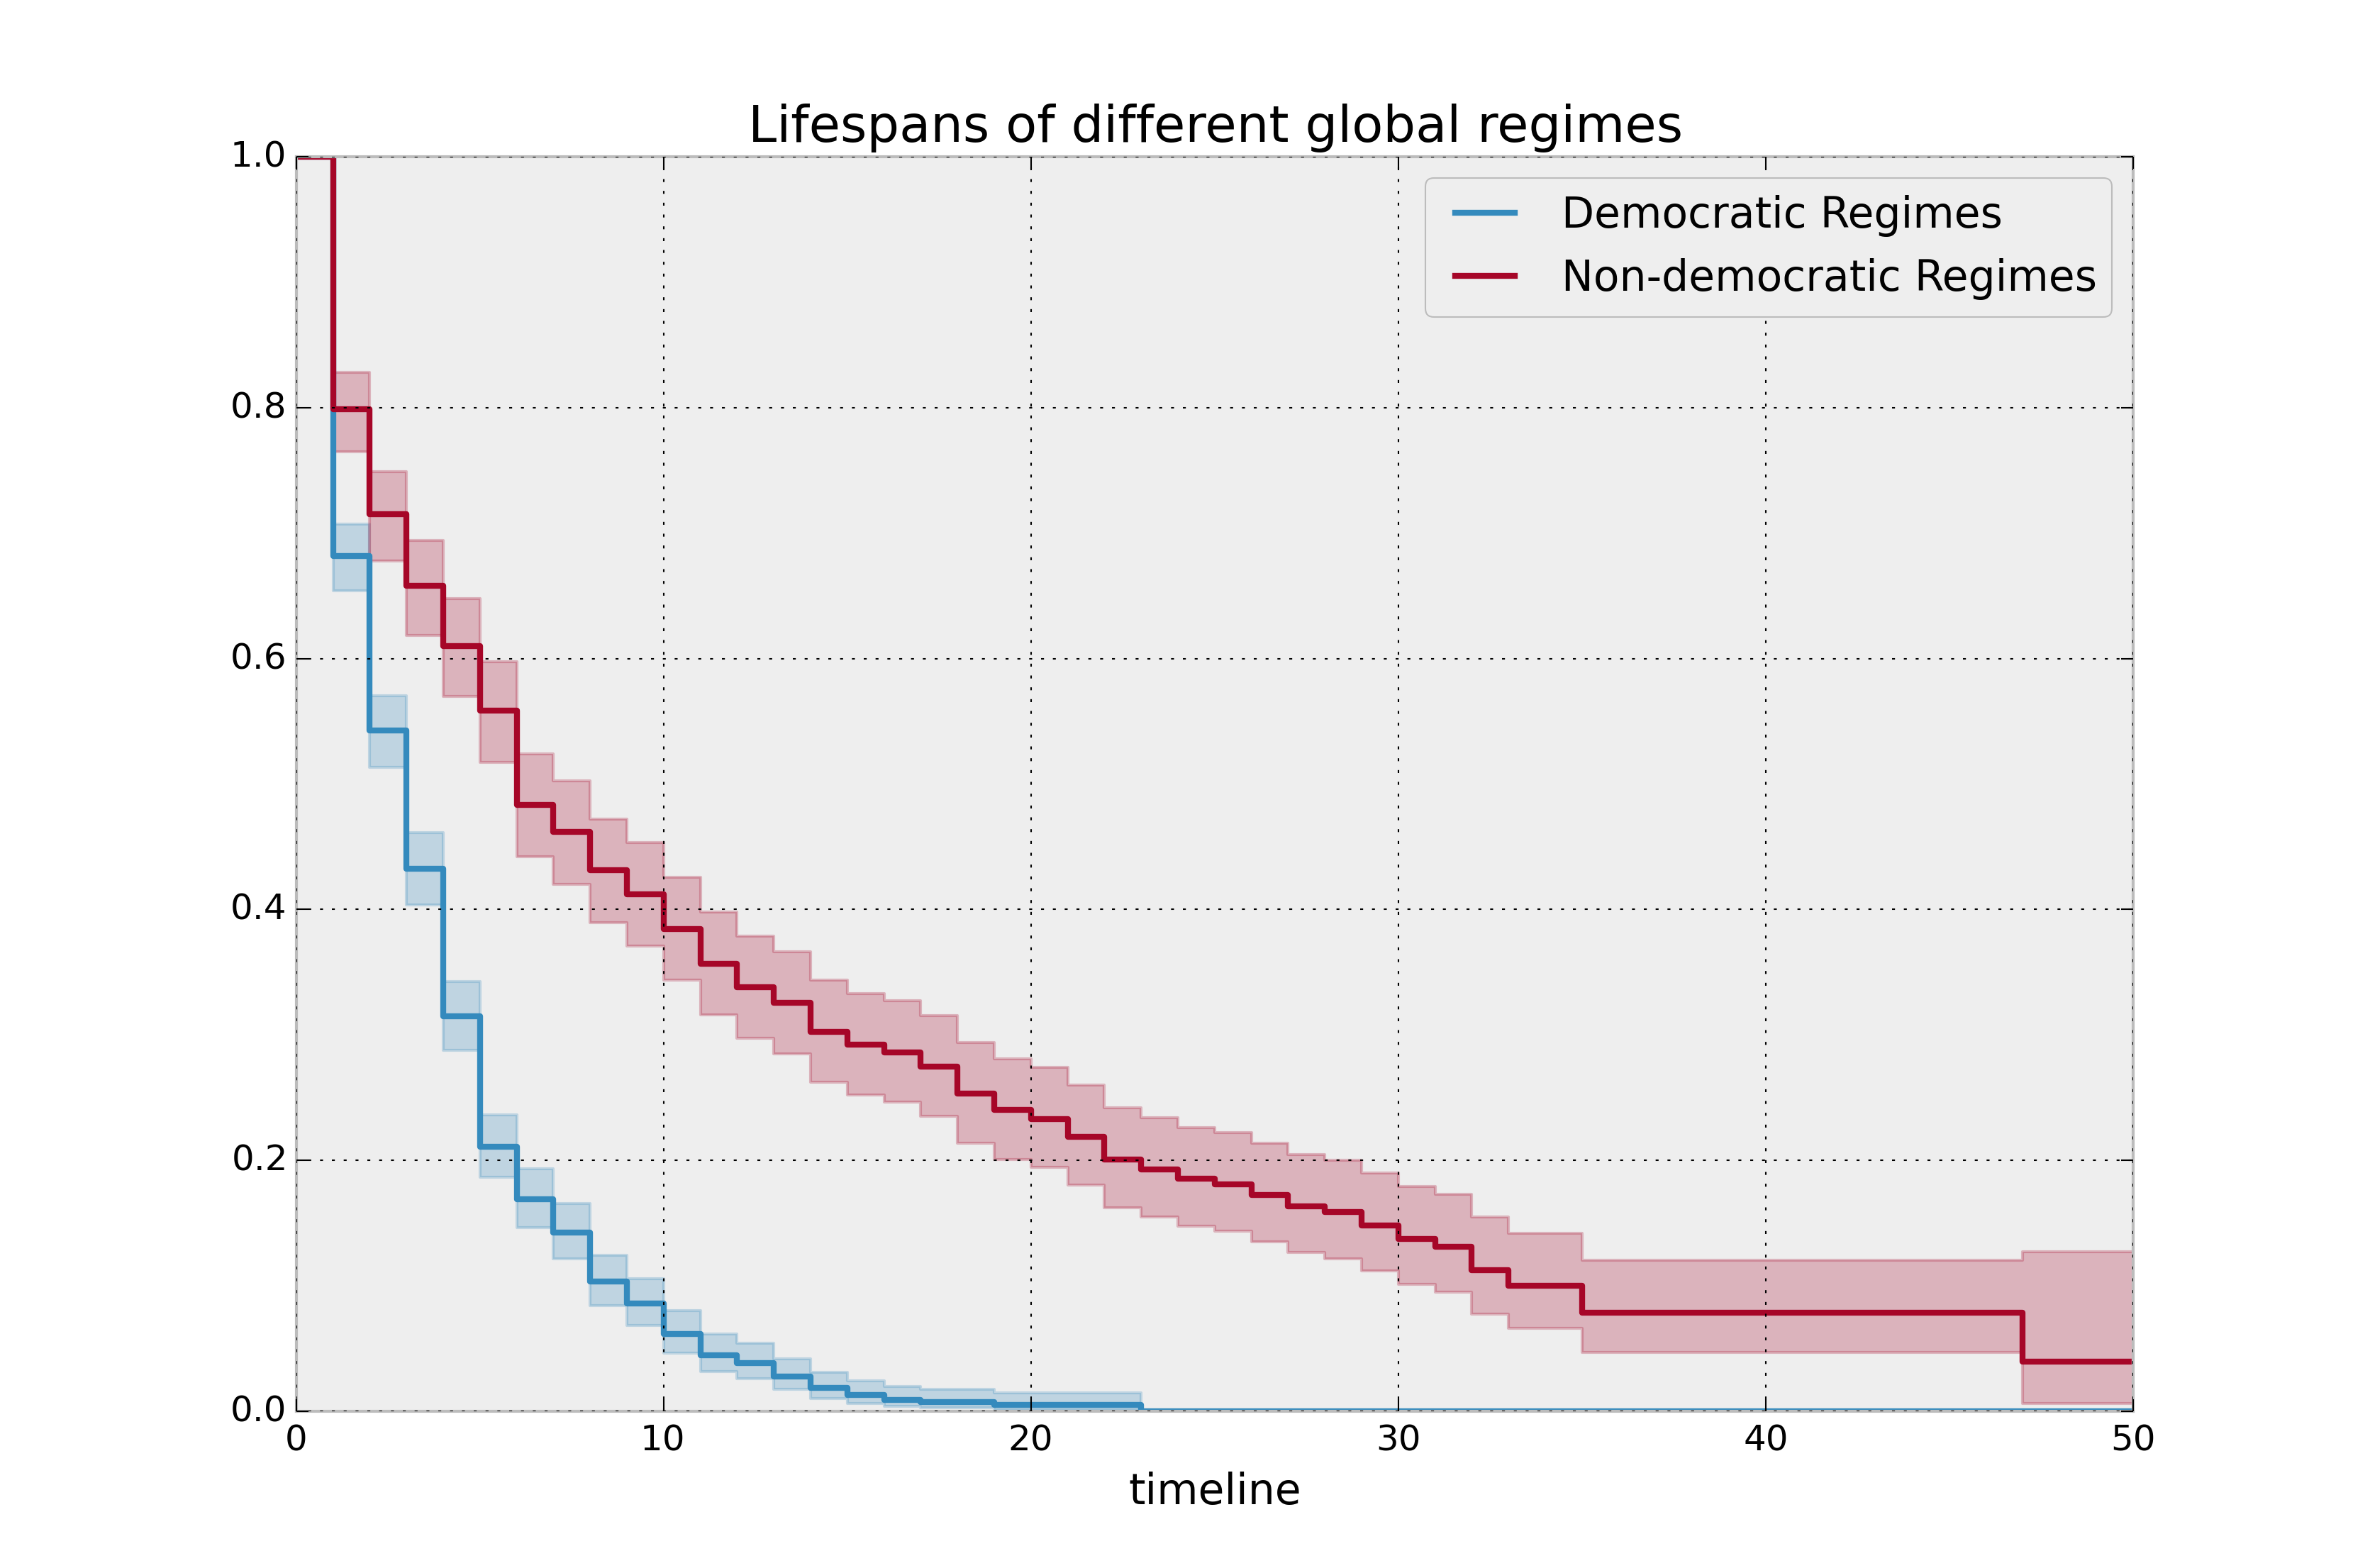
\includegraphics[width=8cm]{lifelines-regimes.png}
		\centering
	\end{figure}
\end{frame}

\begin{frame}
	\begin{itemize}
		\item Rich drivers are more likely to honk faster when they're blocked at an intersection.\footnote{See \cite{diekmann1996social} (but note that $N=57$).}
	\end{itemize}
	\begin{figure}
		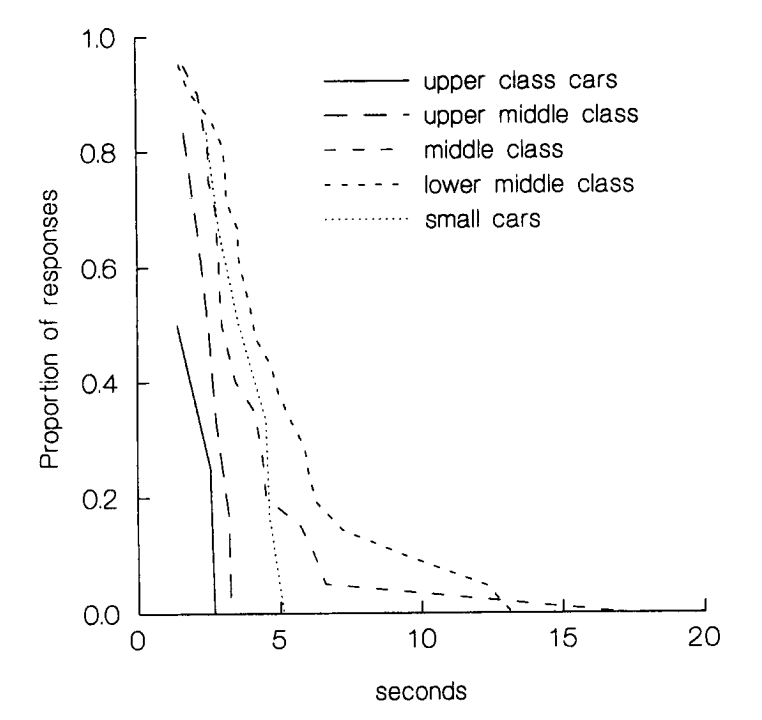
\includegraphics[width=6cm]{diekmann-cars.png}
		\centering
	\end{figure}
\end{frame}

\begin{frame}
	\begin{itemize}
		\item Armand (et al.) used this to look at building safety complaints in Los Angeles.\footnote{\url{latimes.com/local/cityhall/la-me-building-safety-delay-20141219-story.html}}
	\end{itemize}
	\begin{displayquote}
		``Last year, the citywide median wait for a visit from an inspector or other initial action by the building department following a complaint was eight days -- compared with 26 days in the eastern parts of the city.''
	\end{displayquote}
	\begin{figure}
		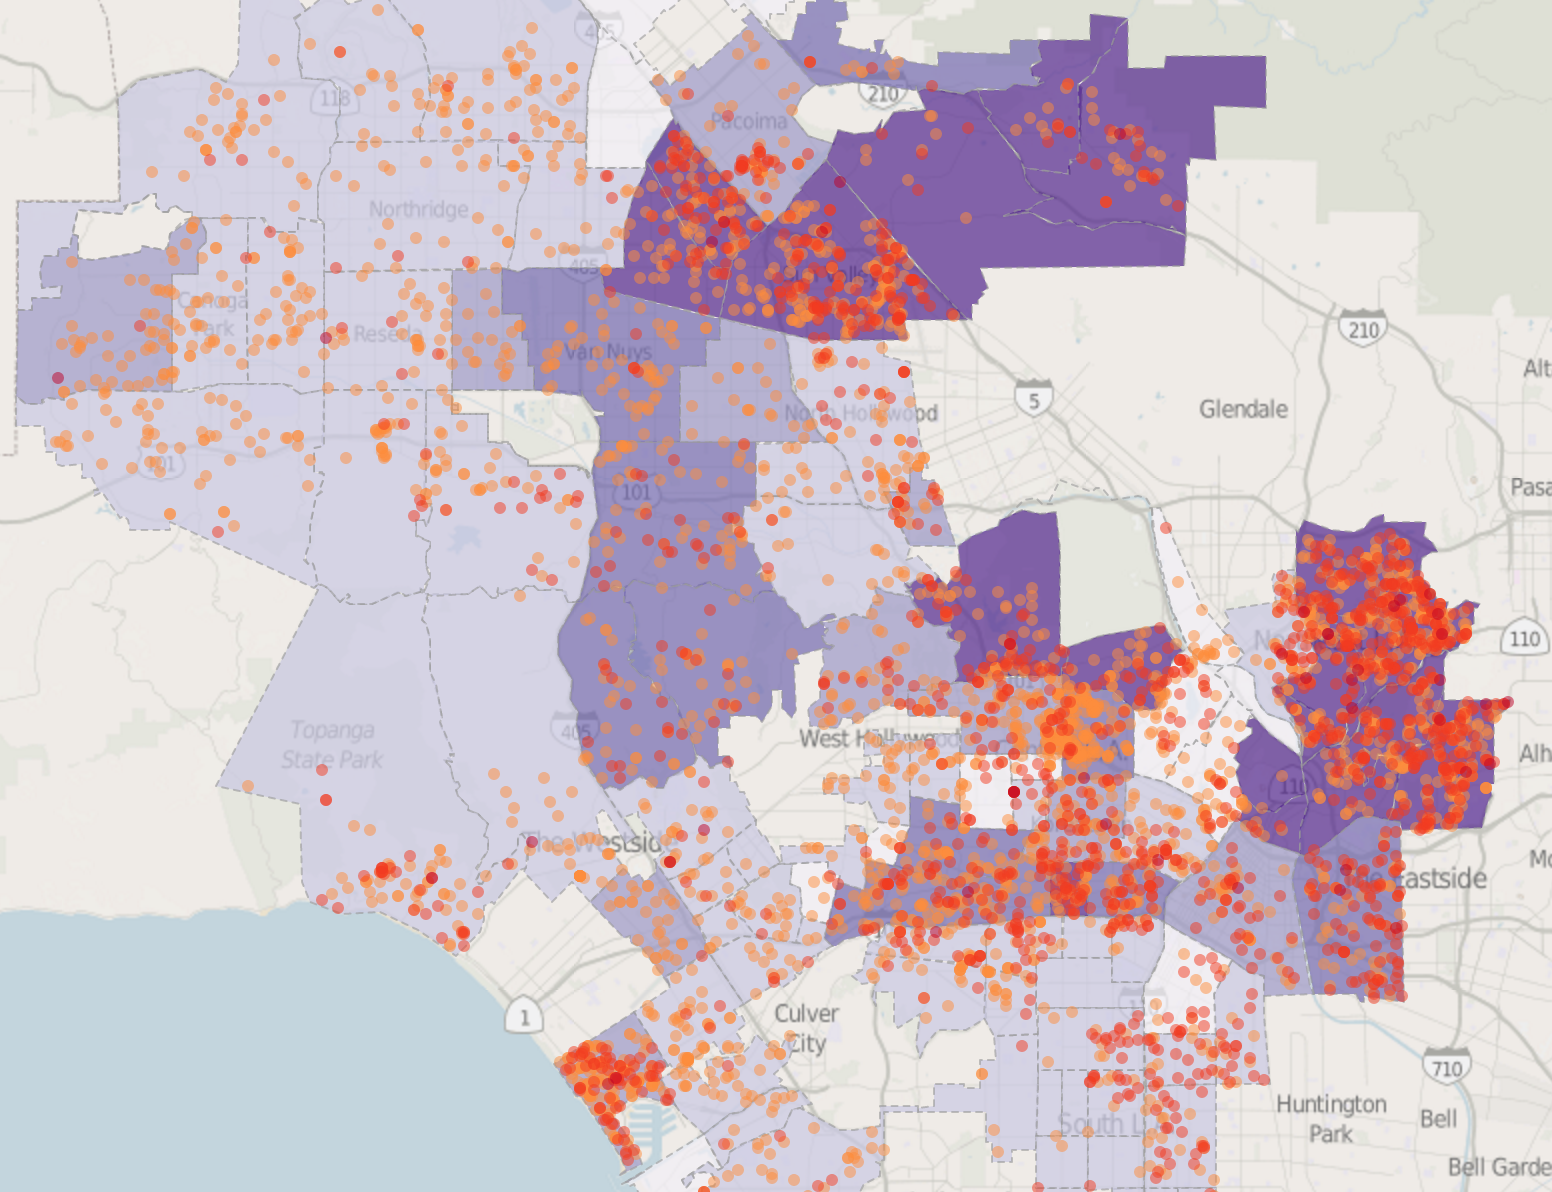
\includegraphics[width=6cm]{latimes-complaints.png}
		\centering
	\end{figure}
\end{frame}

\begin{frame}
	\begin{itemize}
		\item How to do it
		\begin{itemize}
			\item The Python \texttt{lifelines} package is good and well-documented.
			\item Use the \texttt{KaplanMeierFitter} to estimate the survival function and the \texttt{CoxPHFitter} to run a survival regression.
			\item Median lifetime is an intuitive and powerful statistic.\footnote{But nothing is easy, see \cite{singer2003describing} p. 347 for caveats.}
		\end{itemize}
	\end{itemize}
\end{frame}

\section{References}

\begin{frame}[allowframebreaks]
        \bibliographystyle{apalike}
        \bibliography{slides.bib}
\end{frame}

\end{document}